% DPF 09 talk on strangeness in nucleon

\documentclass[10pt]{beamer}
\usepackage{amsmath}
\usefonttheme{professionalfonts} % using non standard fonts for beamer
\usefonttheme{serif} % default family is serif\
\usepackage{mathtools}
%\documentclass[12pt]{beamerthemeSam.sty}
\usepackage{epsf}
%\usepackage{pstricks}
%\usepackage[orientation=portrait,size=A4]{beamerposter}
\geometry{paperwidth=160mm,paperheight=120mm}
%DT favorite definitions
\def\LL{\left\langle}	% left angle bracket
\def\RR{\right\rangle}	% right angle bracket
\def\LP{\left(}		% left parenthesis
\def\RP{\right)}	% right parenthesis
\def\LB{\left\{}	% left curly bracket
\def\RB{\right\}}	% right curly bracket
\def\PAR#1#2{ {{\partial #1}\over{\partial #2}} }
\def\PARTWO#1#2{ {{\partial^2 #1}\over{\partial #2}^2} }
\def\PARTWOMIX#1#2#3{ {{\partial^2 #1}\over{\partial #2 \partial #3}} }

\def\rightpartial{{\overrightarrow\partial}}
\def\leftpartial{{\overleftarrow\partial}}
\def\diffpartial{\buildrel\leftrightarrow\over\partial}

\def\BI{\begin{itemize}}
\def\EI{\end{itemize}}
\def\BE{\begin{displaymath}}
\def\EE{\end{displaymath}}
\def\BEA{\begin{eqnarray*}}
\def\EEA{\end{eqnarray*}}
\def\BNEA{\begin{eqnarray}}
\def\ENEA{\end{eqnarray}}
\def\EL{\nonumber\\}


\newcommand{\map}[1]{\frame{\frametitle{\textbf{Course map}}
\centerline{\includegraphics[height=0.86\paperheight]{../../map/#1.png}}}}
\newcommand{\wmap}[1]{\frame{\frametitle{\textbf{Course map}}
\centerline{\includegraphics[width=0.96\paperwidth]{../../map/#1.png}}}}

\newcommand{\etal}{{\it et al.}}
\newcommand{\gbeta}{6/g^2}
\newcommand{\la}[1]{\label{#1}}
\newcommand{\ie}{{\em i.e.\ }}
\newcommand{\eg}{{\em e.\,g.\ }}
\newcommand{\cf}{cf.\ }
\newcommand{\etc}{etc.\ }
\newcommand{\atantwo}{{\rm atan2}}
\newcommand{\Tr}{{\rm Tr}}
\newcommand{\dt}{\Delta t}
\newcommand{\op}{{\cal O}}
\newcommand{\msbar}{{\overline{\rm MS}}}
\def\chpt{\raise0.4ex\hbox{$\chi$}PT}
\def\schpt{S\raise0.4ex\hbox{$\chi$}PT}
\def\MeV{{\rm Me\!V}}
\def\GeV{{\rm Ge\!V}}

%AB: my color definitions
%\definecolor{mygarnet}{rgb}{0.445,0.184,0.215}
%\definecolor{mygold}{rgb}{0.848,0.848,0.098}
%\definecolor{myg2g}{rgb}{0.647,0.316,0.157}
\definecolor{abtitlecolor}{rgb}{0.0,0.255,0.494}
\definecolor{absecondarycolor}{rgb}{0.0,0.416,0.804}
\definecolor{abprimarycolor}{rgb}{1.0,0.686,0.0}
\definecolor{Red}           {cmyk}{0,1,1,0}
\definecolor{Grey}           {cmyk}{.7,.7,.7,0}
\definecolor{Lg}           {cmyk}{.4,.4,.4,0}
\definecolor{Blue}          {cmyk}{1,1,0,0}
\definecolor{Green}         {cmyk}{1,0,1,0}
\definecolor{Brown}         {cmyk}{0,0.81,1,0.60}
\definecolor{Black}         {cmyk}{0,0,0,1}

\usetheme{Madrid}


%AB: redefinition of beamer colors
%\setbeamercolor{palette tertiary}{fg=white,bg=mygarnet}
%\setbeamercolor{palette secondary}{fg=white,bg=myg2g}
%\setbeamercolor{palette primary}{fg=black,bg=mygold}
\setbeamercolor{title}{fg=abtitlecolor}
\setbeamercolor{frametitle}{fg=abtitlecolor}
\setbeamercolor{palette tertiary}{fg=white,bg=abtitlecolor}
\setbeamercolor{palette secondary}{fg=white,bg=absecondarycolor}
\setbeamercolor{palette primary}{fg=black,bg=abprimarycolor}
\setbeamercolor{structure}{fg=abtitlecolor}

\setbeamerfont{section in toc}{series=\bfseries}

%AB: remove navigation icons
\beamertemplatenavigationsymbolsempty
\title{
  \textbf {Rotational motion}\\
%\centerline{}
%\centering
%\vspace{-0.0in}
%\includegraphics[width=0.3\textwidth]{propvalues_0093.pdf}
%\vspace{-0.3in}\\
%\label{intrograph}
}

\author[W. Freeman] {Physics 211\\Syracuse University, Physics 211 Spring 2015\\Walter Freeman}

\date{\today}

\begin{document}

\frame{\titlepage}

\frame{\frametitle{\textbf{Announcements}}
\BI
\item{Homework deadline extended until Friday}
\item{I should be able to answer all your emails this afternoon}
\item{After the retake, the average on Exam 2 was 70\%}
\EI
}

\frame{\frametitle{\textbf{Rotational motion, summarized}}
\Large
\BI
\item{Force diagrams: draw the entire object, and label at what point the forces act on them}
\item{Choose a pivot (for rotating things, choose the rotation axis}
\item{Newton's law for rotation: $\tau = I \alpha$}
\BI
\item{Applies separately for each rotating object}
\EI
\item{Sometimes you will also need $\vec F = m \vec a$}
\item{For static equilibrium problems: $\alpha = 0$}
\EI
}


\frame{\frametitle{\textbf{Statics problems}}
\Large
\BI
\item{Often we know $\alpha = \vec a = 0$}
\item{This tells us that the net torque (about {\it any} pivot) and the net force are both zero}
\item{Usually this is because an object isn't moving, but sometimes it's moving at a constant rate (tomorrow's recitation problem)}
\item{Plan of attack:}
\BI
\item{Compute the torque about any point and set it to zero}
\item{Choose a pivot conveniently at the location of a force we don't care about}
\item{If needed, also write $\sum \vec F = 0$}
\EI
\EI
}

\frame{\frametitle{\textbf{When do objects balance?}}
\Large
\BI
\item{Remember normal forces can only push, never pull}
\item{Think about what happens as something begins to tip}
\item{As an object topples over, its entire weight rests on the corner of the surface...}
\EI
}

\frame{\frametitle{\textbf{Statics problems: a sample}}
\large
\BI
\item{What is the weight of the bar?}
\pause
\item{How does the force needed to support it depend on the angle of the force?}
\pause
\item{How does the force needed to support it depend on the angle of the bar?}
\pause
\item{What if I hang weights from it?}
\EI
}

\frame{\frametitle{\textbf{Balance problems: a sample}}
\Large
How far can I walk out onto the plank before it falls?

\bigskip
\pause

How does a balance beam work? How do we weigh objects with one?

\bigskip
\pause

Which of these can drive up a snowy hill more easily?

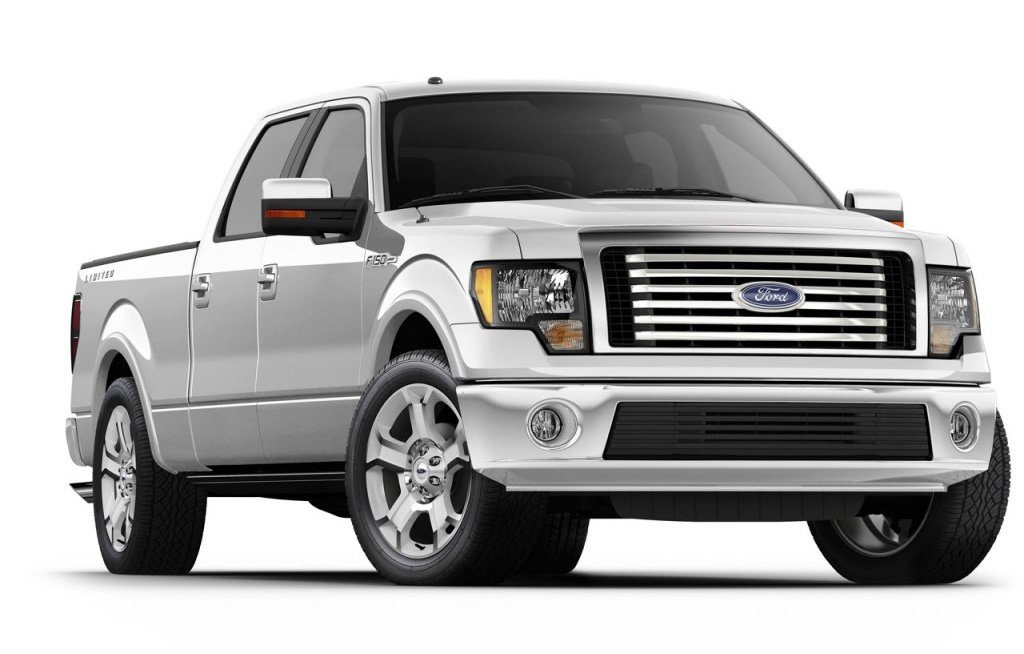
\includegraphics[width=0.5\textwidth]{truck.jpg}
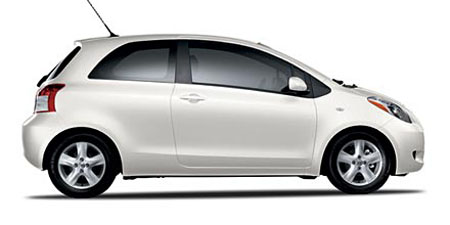
\includegraphics[width=0.5\textwidth]{yaris.jpg}



}
\frame{\frametitle{\textbf{Rotational dynamics: gears}}
\Large
Consider two gears: one with a radius r, one with a radius R, touching each other.

If they turn at constant angular velocity, and a torque $\tau_1$ is applied to gear 1, what torque can gear 2 apply to something else?

\BI
\item{How are their tangential velocities related?}
\pause
\item{How are their angular velocities related?}
\pause
\item{How does the power applied to each relate?}
\pause
\item{This problem is very similar to problem 6 on your homework!}
\EI
}


\frame{\frametitle{\textbf{Rotational dynamics: how do gears work?}}
\large
\BI
\item{Two touching gears or wheels apply the same force of static friction to each other}
\item{Their tangential velocities are also the same}
\item{If their radii are different, this allows you to trade angular velocity for torque}
\EI
\begin{align*}
F_1 &= F_2 \rightarrow \frac{\tau_1}{\tau_2} = \frac{r_1}{r_2} \\
v_{T,1} &= v_{T,2} \rightarrow \omega_1 r_1 = \omega_2 r_2 \rightarrow \frac{\omega_1}{\omega_2} = \frac{r_2}{r_1}
\end{align*}
}

\end{document}
